\documentclass[xcolor=dvipsname,handout]{beamer} %handout, ignorenonframetext

%\usepackage[ngerman]{babel}
\usepackage[utf8]{inputenc}
\usepackage{amsmath} 
\usepackage{graphicx} 
\usepackage{subfigure} 
\usepackage{multimedia}
\usepackage{wrapfig}
\usepackage{listings}
\usepackage{comment}
\usepackage{framed,color}
\usepackage{listings}


\fboxsep=1pt%padding thickness
\fboxrule=1pt%border thickness
\usepackage{fancybox}

\usepackage{lipsum}
\usepackage{tabularx}
\usepackage{colortbl}
\usepackage{url}


\hypersetup{
	linkcolor=DarkSkyBlue,
	citecolor= DarkSkyBlue,
	filecolor= DarkSkyBlue,
	urlcolor= DarkSkyBlue
}


% COLOR-DEFINITION
%%%%%%%%%%%%%%%%%%%%%%%%
\definecolor{LightButter}{rgb}{0.98,0.91,0.31}
\definecolor{LightOrange}{rgb}{0.98,0.68,0.24}
\definecolor{LightChocolate}{rgb}{0.91,0.72,0.43}
\definecolor{LightChameleon}{rgb}{0.54,0.88,0.20}
\definecolor{LightSkyBlue}{rgb}{0.45,0.62,0.81}
\definecolor{LightPlum}{rgb}{0.68,0.50,0.66}
\definecolor{LightScarletRed}{rgb}{0.93,0.16,0.16}
\definecolor{LightGray}{rgb}{0.80,0.80,0.80}
\definecolor{Butter}{rgb}{0.93,0.86,0.25}
\definecolor{Orange}{rgb}{0.96,0.47,0.00}
\definecolor{Chocolate}{rgb}{0.75,0.49,0.07}
\definecolor{Chameleon}{rgb}{0.45,0.82,0.09}
\definecolor{SkyBlue}{rgb}{0.20,0.39,0.64}
\definecolor{Plum}{rgb}{0.46,0.31,0.48}
\definecolor{ScarletRed}{rgb}{0.80,0.00,0.00}
\definecolor{DarkButter}{rgb}{0.77,0.62,0.00}
\definecolor{DarkOrange}{rgb}{0.80,0.36,0.00}
\definecolor{DarkChocolate}{rgb}{0.56,0.35,0.01}
\definecolor{DarkChameleon}{rgb}{0.30,0.60,0.02}
\definecolor{DarkSkyBlue}{rgb}{0.12,0.29,0.53}
\definecolor{DarkPlum}{rgb}{0.36,0.21,0.40}
\definecolor{DarkScarletRed}{rgb}{0.64,0.00,0.00}



% HPI-THEME
%%%%%%%%%%%%%%%%%%%%%%%%
\RequirePackage{scrlfile}
%\ReplaceFile{beamerthemehpiswa.sty}{theme/beamerthemehpiswa.sty}
%\ReplaceFile{beamercolorthemehpiswa.sty}{theme/beamercolorthemehpiswa.sty}
%\ReplaceFile{beamerfontthemehpiswa.sty}{theme/beamerfontthemehpiswa.sty}
%\ReplaceFile{beamerinnerthemehpiswa.sty}{theme/beamerinnerthemehpiswa.sty}
%\ReplaceFile{beamerouterthemehpiswa.sty}{theme/beamerouterthemehpiswa.sty}
%\ReplaceFile{hpi.png}{theme/hpi.png}
\usetheme{hpiswa}


% BEAMER-Anpassungen
%%%%%%%%%%%%%%%%%%%%%%%%
\setbeamercolor{block title}{bg=DarkOrange}
\setbeamercolor{block body}{bg=Orange!20} 
%\setbeamercolor{block title alerted}{bg=red}
\setbeamercolor{block body alerted}{bg=red!20} 
%\setbeamercolor{block title example}{bg=green}
\setbeamercolor{block body example}{bg=DarkChameleon!20} 
%\usecolortheme[RGB={205,173,0}]{structure} 
\usecolortheme[RGB={30,74,135}]{structure}

\usecolortheme{orchid}
%\usefonttheme{professionalfonts}
%\useoutertheme[subsection=false]{smoothbars}
%\useinnertheme{rectangles}
%\setbeamertemplate{blocks}[shadow=true] 

\setbeamercovered{transparent}
\setbeamertemplate{navigation symbols}{}%remove navigation symbols



% Eigene Anpassungen
%%%%%%%%%%%%%%%%%%%%

% Explainframes:
\usepackage{ifthen}
\newboolean{isexplainframe}
\setboolean{isexplainframe}{false}
\mode<handout>{
\newenvironment{explainframe}[1]{
\setboolean{isexplainframe}{true}
\addtocounter{framenumber}{-1}
\setbeamertemplate{background}[grid][step=5mm,color=LightGray]
\begin{frame}{Handout only: #1}%
}{%
\end{frame}%
\setboolean{isexplainframe}{false}
}}
\mode<beamer>{
\excludecomment{explainframe}
}

\setbeamertemplate{footline}{%
	\leavevmode%
	\hbox{%
		\begin{beamercolorbox}[wd=.333333\paperwidth,ht=2.25ex,dp=1ex,center]{author in head/foot}%
			\usebeamerfont{author in head/foot}\insertinstitute
		\end{beamercolorbox}%
		\begin{beamercolorbox}[wd=.333333\paperwidth,ht=2.25ex,dp=1ex,center]{title in head/foot}%
			\usebeamerfont{title in head/foot}\insertshorttitle
		\end{beamercolorbox}%
		\begin{beamercolorbox}[wd=.333333\paperwidth,ht=2.25ex,dp=1ex,right]{date in head/foot}%
			\usebeamerfont{date in head/foot}\insertshortdate{}\hspace*{2em}
			\insertframenumber{}\ifthenelse{\boolean{isexplainframe}}{E}{} / \inserttotalframenumber\hspace*{2ex}
	\end{beamercolorbox}}%
	\vskip0pt%
}

\definecolor{javared}{rgb}{0.6,0,0} % for strings
\definecolor{javagreen}{rgb}{0.25,0.5,0.35} % comments
\definecolor{javapurple}{rgb}{0.5,0,0.35} % keywords
\definecolor{javadocblue}{rgb}{0.25,0.35,0.75} % javadoc

\lstset{
  language=Ruby,
  basicstyle=\scriptsize\ttfamily,
  keywordstyle=\color{javapurple}\bfseries,
  stringstyle=\color{javared},
  commentstyle=\color{javagreen},
  morecomment=[s][\color{javadocblue}]{/**}{*/},
  tabsize=4,
  showspaces=false,
  showstringspaces=false,
  breaklines=true
}


% Gliederung vor jedem Punkt:
\AtBeginSection[]{
\ifthenelse{\equal{\value{section}}{1}}{}{
\begin{frame}{Overview}
	\tableofcontents[currentsection, hideothersubsections]
\end{frame}
}
}


% Quote-Environment:

\renewenvironment{quote}{%
\begin{exampleblock}{}%
\begin{center}%
\begin{large}%
``}{%
''\end{large}%
\end{center}%
\end{exampleblock}}




% Dokument-Meta-Daten:
%%%%%%%%%%%%%%%%%%%%%%%
\title{Truffle -- an overview}
\subtitle{Virtual Machines and Execution Environments, WS2014/15}
\author{Jan Graichen, Fabio Niephaus, Matthias Springer, Malte Swart}
\date{\today}
\institute[2012]{Hasso Plattner Institute, Software Architecture Group}



\begin{document}

\begin{frame}[plain]
	\maketitle
\end{frame}
\begin{frame}{Overview}
	\tableofcontents[hideallsubsections]
\end{frame}

\section{Keyword Arguments}

\begin{frame}[fragile]{Keyword Arguments in Ruby 2.0}
\begin{lstlisting}
def method(a, b = 1, c:, d: 2, **more)
    [a, b, c, d]
end

method(10, e: 30, c: 40)
=> [10, 1, 40, 2]
\end{lstlisting}

\begin{table}
    \centering
    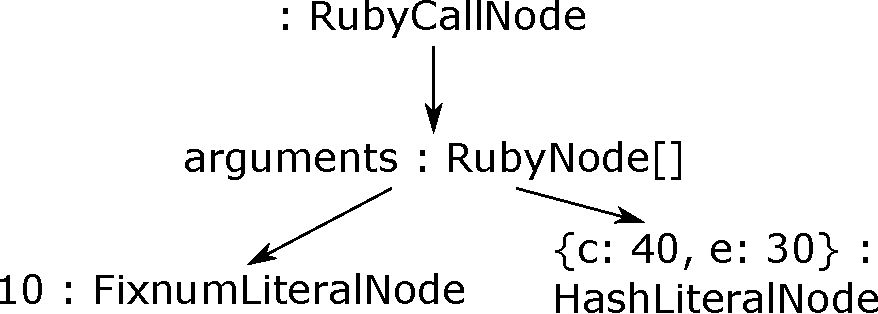
\includegraphics[width=0.75\textwidth]{kwarg_1.pdf}
\end{table}
\end{frame}

\begin{frame}[fragile]{Keyword Arguments in Ruby 2.0}
\begin{lstlisting}
def method(a = 1, b: 2)
    [a, b]
end

method({b: 3})
=> [1, 3]
\end{lstlisting}
\end{frame}

\begin{frame}[fragile]{Keyword Arguments in Ruby 2.0}
\begin{lstlisting}
def method(a = 1, b: 2)
    [a, b]
end

method({x: 1})
ArgumentError: unknown keyword: x
\end{lstlisting}
\end{frame}

\begin{frame}{JRuby: Implementation of Keyword Arguments}
\begin{table}
    \centering
    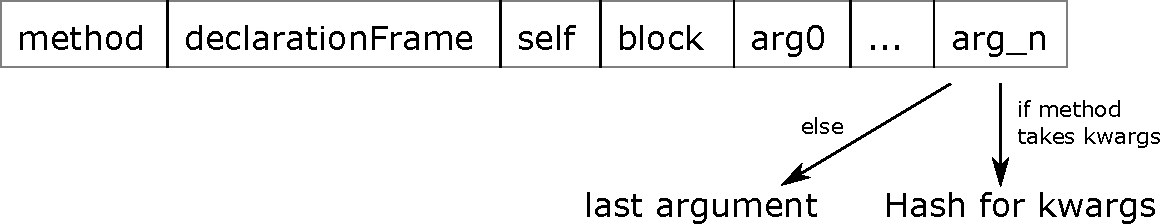
\includegraphics[width=\textwidth]{method_args_array.pdf}
\end{table}

\begin{itemize}
    \item Parser generates \lstinline{HashNode} for keyword argument
    \item Keyword arguments are stored in last argument in arguments array
\end{itemize}
\end{frame}

\begin{frame}{JRuby Compilation Process}
\begin{enumerate}
    \item Ruby Source Code
    \item JRuby AST
    \item JRuby Truffle AST (with specializations, support for node rewriting)
    \item Byte Code
    \item Native Code 
\end{enumerate}
\end{frame}

\section{Optimizations}
\begin{frame}{Was Malte macht}

\end{frame}

\begin{frame}{Store Keyword Arguments in Array}
\begin{itemize}
    \item Before: \lstinline{RubyCallNode.arguments} contains a Hash as last array element
    \item Idea: add key-value pairs to array with marker object as hash separator
    \item Benefit: no Hash creation
\end{itemize}

\begin{table}
\begin{tabular}{|c|c|c|c|c|c|c|c|c|c|}
\hline
$\mathit{arg}_1$ & \ldots & $\mathit{arg}_{n-1}$ & * & $\mathit{key}_1$ & $\mathit{value}_1$ & $\mathit{key}_2$ & $\mathit{value}_2$ & \ldots & * \\
\hline
\end{tabular}
\end{table}
\begin{itemize}
    \item $\mathit{arg}_i$: $i$th argument (\lstinline{RubyNode})
    \item *: marker (\lstinline{MarkerNode}, executes to singleton \lstinline{Object})
    \item $\mathit{key}_i$: $i$th key in Hash (\lstinline{StringLiteralNode})
    \item $\mathit{value}_i$: $i$th value in Hash (\lstinline{RubyNode})
\end{itemize}
\end{frame}

\begin{frame}{Store Keyword Arguments in Array}
\begin{table}
\begin{tabular}{|c|c|c|c|c|}
\hline
method & declarationFrame & self & block & countKwArgs  \\ 
\hline
\end{tabular}
\end{table}
\begin{table}
\begin{tabular}{|c|c|c|c|c|}
\hline
 $\mathit{arg}_0$ & \ldots & $\mathit{arg}_{n-1}$ & *  & $\mathit{key}_1$\\
\hline
\end{tabular}
\end{table}

\begin{table}
\begin{tabular}{|c|c|c|c|c|}
\hline
 $\mathit{value}_1$ & \ldots  & $\mathit{key}_m$ & $\mathit{value}_m$ & * \\
\hline
\end{tabular}
\end{table}

\begin{itemize}
    \item $\mathit{arg}_i$: $i$th argument (\lstinline{Object})
    \item *: marker (singleton \lstinline{Object})
    \item $\mathit{key}_i$: $i$th key in Hash (\lstinline{String})
    \item $\mathit{value}_i$: $i$th value in Hash (\lstinline{Object})
\end{itemize}
\end{frame}

\begin{frame}{Store Keyword Arguments in Array}
\begin{itemize}
    \item Read keyword argument: if \lstinline{countKwArgs > 0}, scan expanded Hash. Else, extract value from Hash.
    \item Read argument: if last argument is expanded Hash: \\ generate Hash object.
    \item Read rest keyword arguments: generate Hash object for keywords that are not excluded.
\end{itemize}
\end{frame}

\begin{frame}{Recap: Type Decision Chains}

\end{frame}

\begin{frame}{Fully Optimized Keyword Arguments}
\begin{itemize}
    \item Before: \lstinline{RubyCallNode.arguments} contains keys and values of keyword arguments
    \item Idea: call node is method-specific and stores values only (no keys!) for arguments specified in signature
    \item Benefit: no linear scan of keyword argument array section
\end{itemize}
\end{frame}

\begin{frame}[fragile]{Fully Optimized Keyword Arguments (Example)}
\begin{lstlisting}
class Cls1
    def method(a:, **kwargs)
    end
end

def Cls2
    def method(a:, b:)
    end
end

def getObject
    # first call returns "Cls1.new"
    # second call returns "Cls2.new"
end

2.times do
    getObject().method(a: 1, b: 2)
end
\end{lstlisting}
\end{frame}

\begin{frame}{Fully Optimized Keyword Arguments (Example)}{Type Decision Chain}
\begin{table}
    \centering
    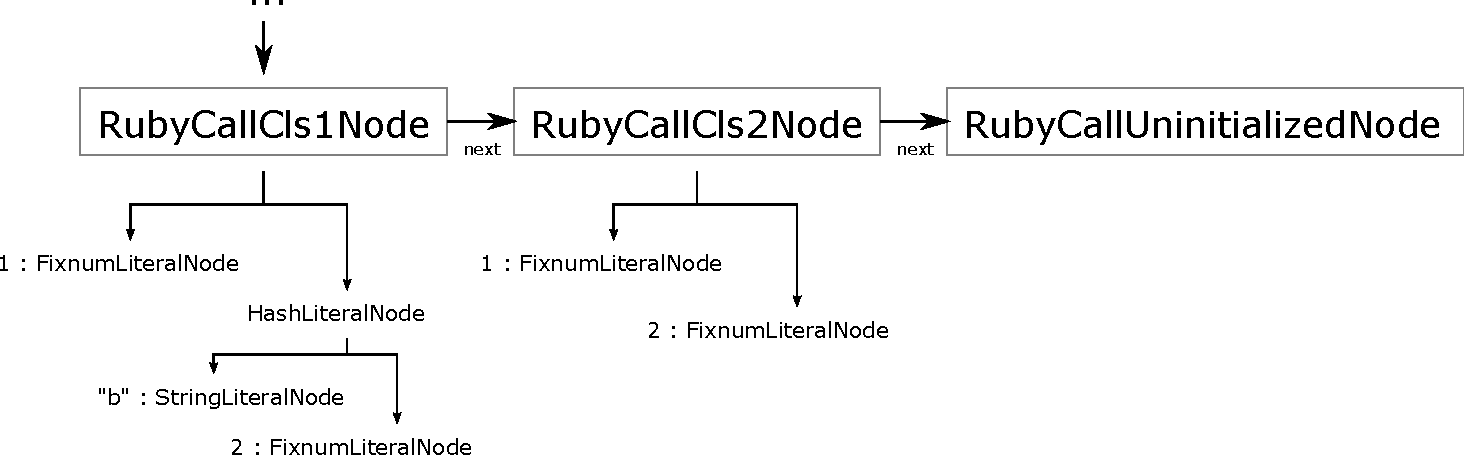
\includegraphics[width=\textwidth]{fully_opt.pdf}
\end{table}

\begin{itemize}
    \item Node specialization for every method (for every receiver type)
    \item Specialized nodes do not construct Hash nodes only to read arguments from them
\end{itemize}
\end{frame}

\begin{frame}{Fully Optimized Keyword Arguments (Example)}{Generic Case}
\begin{table}
    \centering
    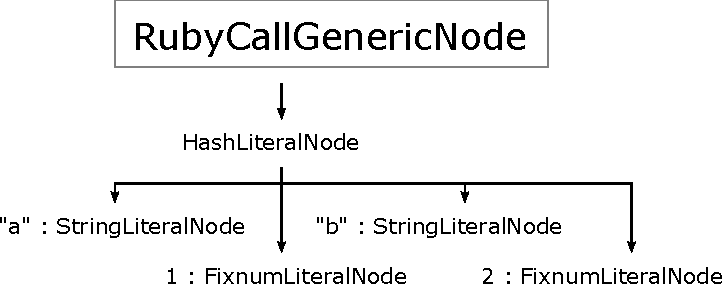
\includegraphics[width=\textwidth]{kwargs_generic.pdf}
\end{table}
\end{frame}

\begin{frame}{Fully Optimized Keyword Arguments}{Problems}
\begin{itemize}
    \item Nodes are specific with regard to user-defined Ruby classes \\ (cannot use Truffle DSL)
    \item Specializations are defined in Java code \\ (need to generate Java classes on the fly)
    \item Type of receiver is not known before dispatching the call
\end{itemize}
\end{frame}

\begin{frame}{Almost Fully Optimized Keyword Arguments}
Store HashMap mapping receiver type to arguments array in RubyCallNodes. Assumption invalidates arguments when method with that name changes. When threshold is reached, switch to old behavior. Kind of specialization built by ourselves.
\end{frame}
\end{document}
